\documentclass[varwidth=\maxdimen]{standalone}

\usepackage{tikz}
\usepackage{graphicx}
\tikzset{every picture/.style={/utils/exec={\sffamily}}}


\begin{document}
\begin{figure}
	\begin{tikzpicture}
	
	\Large

	\begin{scope}[shift={(10,-10)}]
		\node [anchor=south west] (seis) at (0,0) {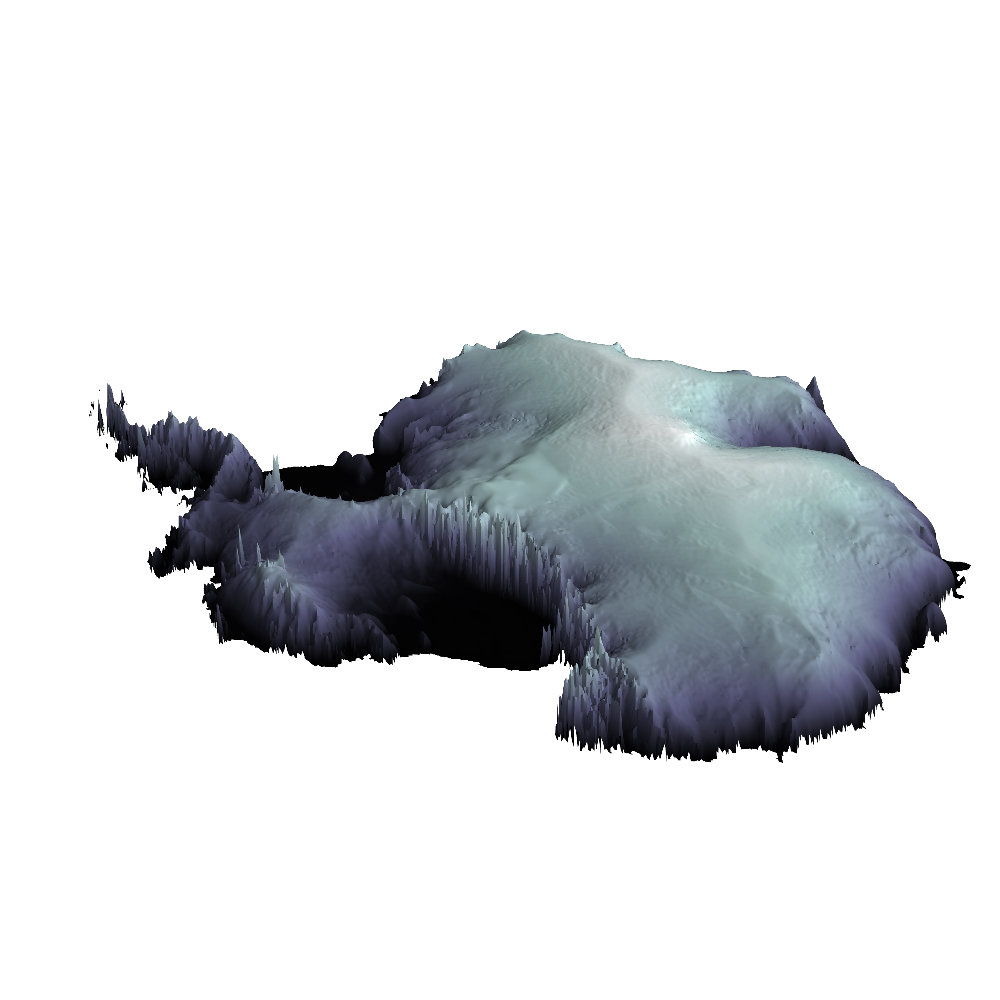
\includegraphics[height=11.5cm] {../fig/oblique_view}};
		\node [] at (0.6,9.0){\textbf{d})};
	\end{scope}



	\begin{scope}[shift={(0,0)}]
		\node [anchor=south west] (seis) at (0,0) {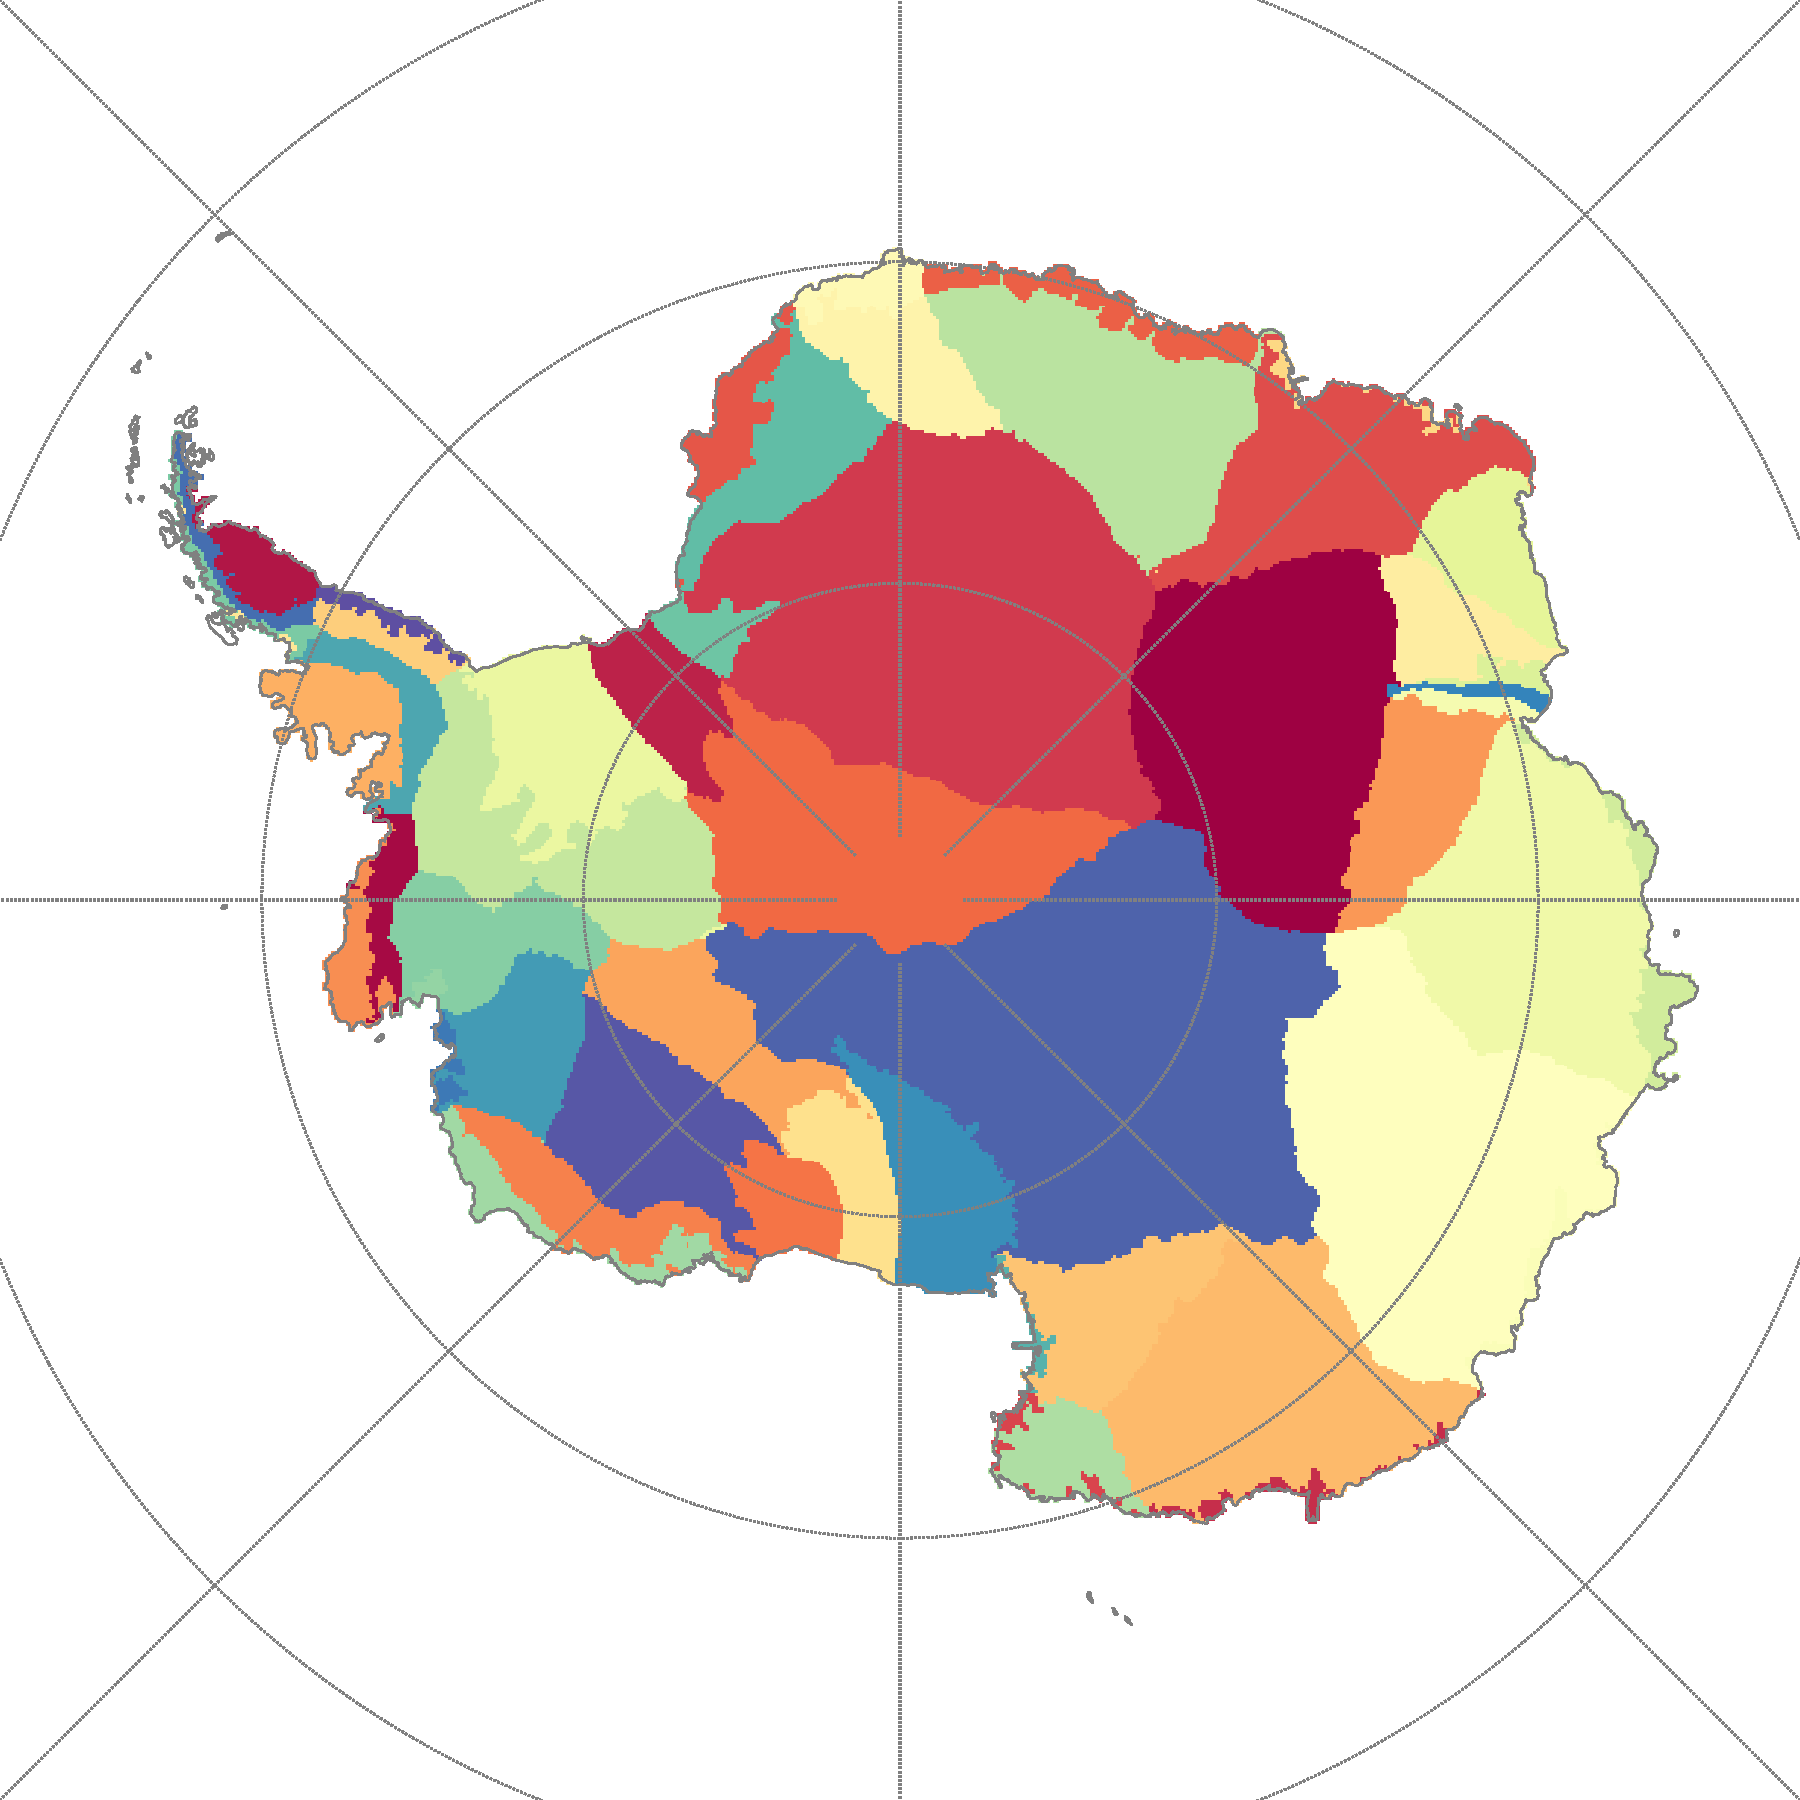
\includegraphics[height=10cm] {../fig/dranage}};
		\node [] at (0.6,9.0){\textbf{a})};
	\end{scope}


	\begin{scope}[shift={(10,0)}]
		\node [anchor=south west] (seis) at (0,0) {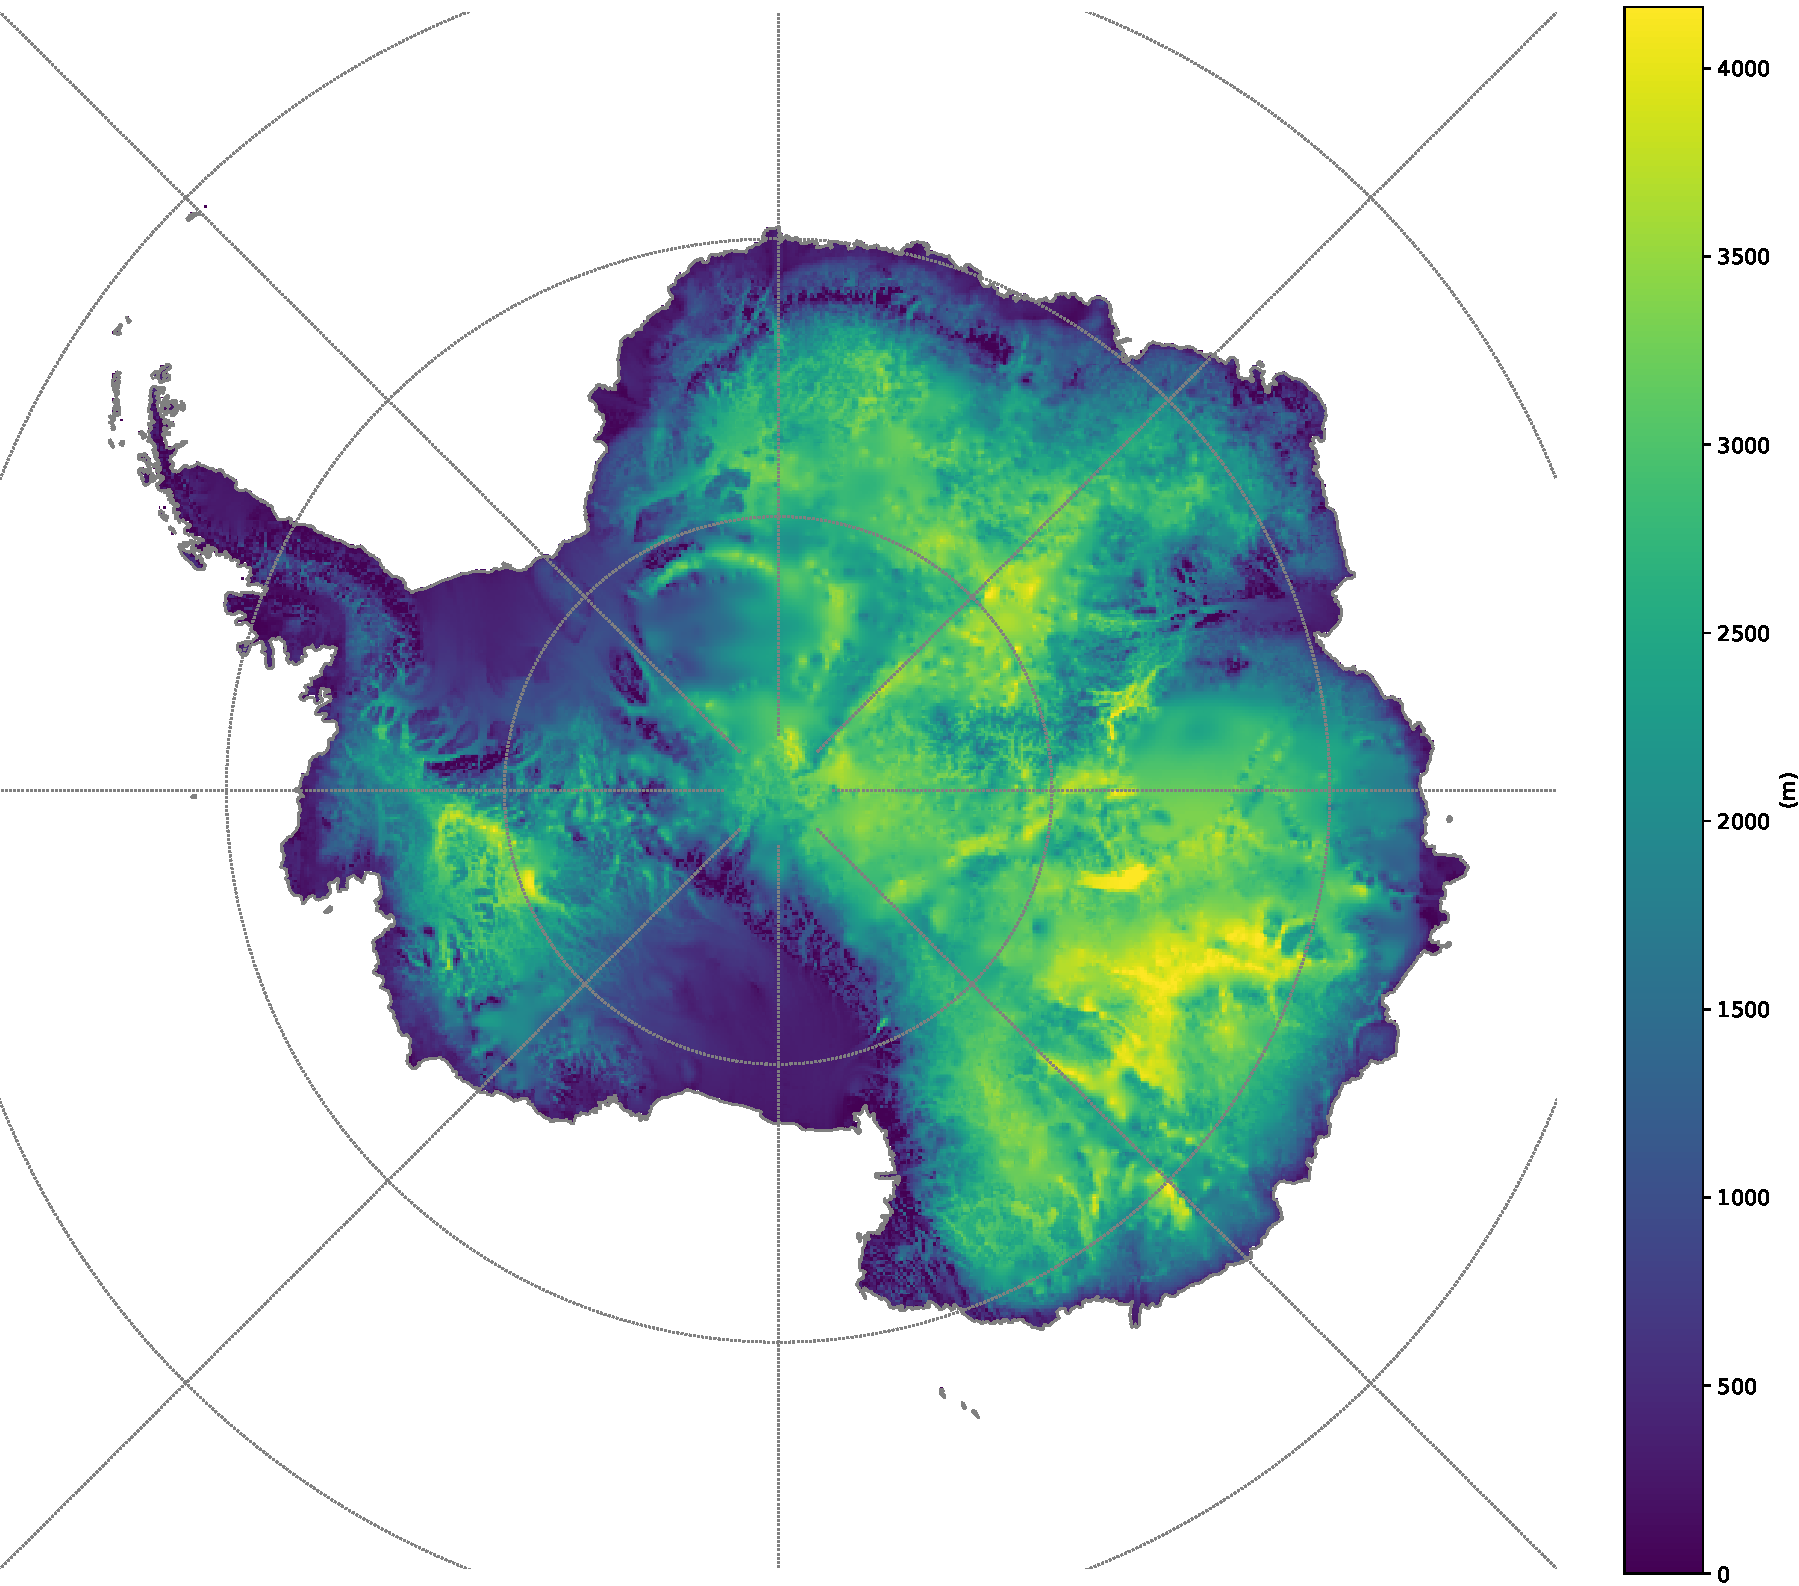
\includegraphics[height=10cm] {../fig/ice}};
		\node [] at (0.6,9.0){\textbf{b})};
	\end{scope}


	\begin{scope}[shift={(0,-10)}]
		\node [anchor=south west] (seis) at (0,0) {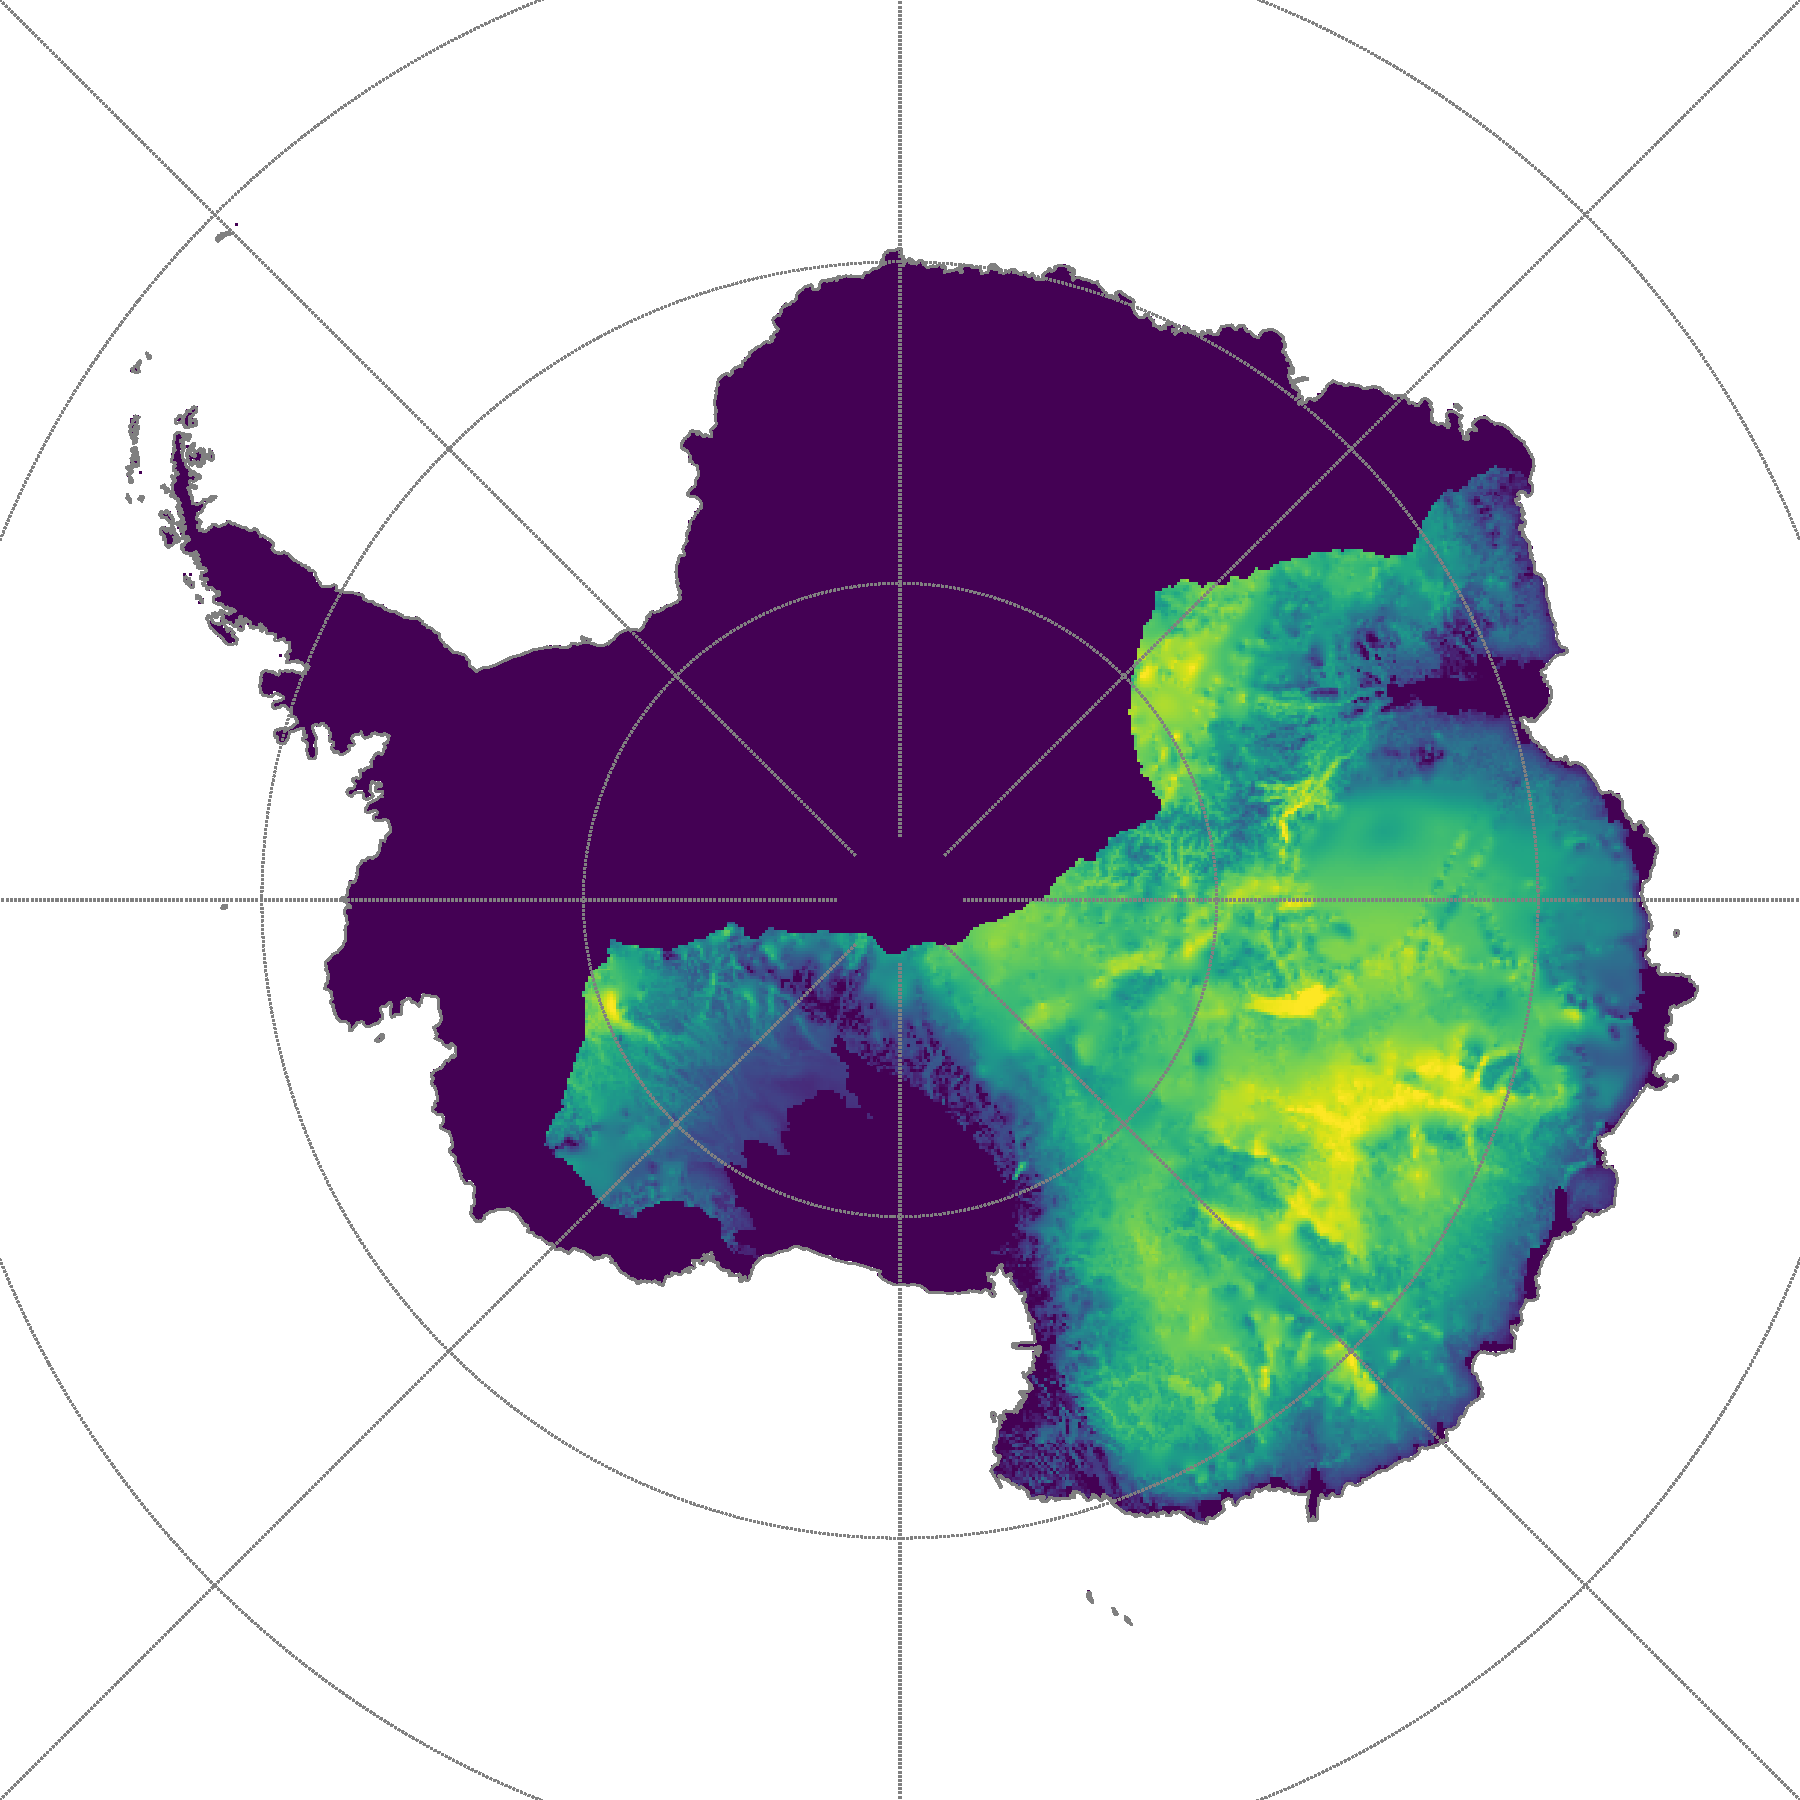
\includegraphics[height=10cm] {../fig/selected}};
		\node [] at (0.6,9.0){\textbf{c})};
	\end{scope}



	\end{tikzpicture}
\end{figure}
\end{document}